\documentclass{sig-alternate}
\usepackage{color}
\usepackage[colorinlistoftodos]{todonotes}
\usepackage{algorithm}
\usepackage[noend]{algpseudocode}



%%%%% Uncomment the following line and comment out the previous one
%%%%% to remove all comments
%%%%% NOTE: comments still occupy a line even if invisible;
%%%%% Don't write them as a separate paragraph
%\newcommand{\mycomment}[1]{}

\begin{document}

\conferenceinfo{UMM CSci Senior Seminar Conference, April 2017}{Morris, MN}

\title{Conflict-Free Vertex Coloring Of Planar Graphs}

\numberofauthors{1}

\author{
\alignauthor
Shawn S. Seymour\\
	\affaddr{Division of Science and Mathematics}\\
	\affaddr{University of Minnesota, Morris}\\
	\affaddr{Morris, Minnesota, USA 56267}\\
	\email{seymo079@morris.umn.edu}
}

\maketitle
\begin{abstract}
The conflict-free coloring problem is a variation of the vertex coloring problem, a classical NP-hard optimization problem. The conflict-free coloring problem aims to color the vertices of a graph in a way where every vertex is connected to at least one uniquely colored vertex. This paper presents heuristics to solve the conflict-free coloring problem on both general graphs and planar graphs. This paper also looks into bounds on the number of colors needed.
\end{abstract}

\section{Introduction}
\label{sec:introduction}

Consider the map of the 48 contiguous states in the United States of America. Suppose we would like to color each state such that no two states that share a boundary have the same color. This problem can be modeled with a graph. We can represent each state with a \emph{vertex} and represent a boundary between two states with an \emph{edge}. This map is an example of a planar graph, i.e. none of the edges cross when drawn on a plane.

This is a famous example of the \emph{vertex coloring} problem and one of many graph coloring problems. The vertex coloring problem aims to find the minimum number of colors needed to color a graph such that no two adjacent vertices are colored with the same color. While some problems are relatively easy to solve, the vertex coloring problem is one of the most computationally complex problems in computer science and mathematics. The vertex coloring problem has many real-world applications such as exam timetabling, register allocation, and the scheduling of taxis.

The \emph{conflict-free coloring} problem is a relaxed variation of the vertex coloring problem. The conflict-free coloring problem does not aim to color every vertex such that it is not connected to a vertex of the same color. Rather, it aims to color \emph{enough} vertices such that for every vertex, it is connected to at least one uniquely colored vertex.


\section{Background}
\label{sec:background}
To understand the problem, the algorithms to solve it, and its results, we must first understand some graph theory, some computational complexity theory, and the precise definitions of the vertex coloring problem and the conflict-free coloring problem.

\begin{figure}[h]
	\centering
	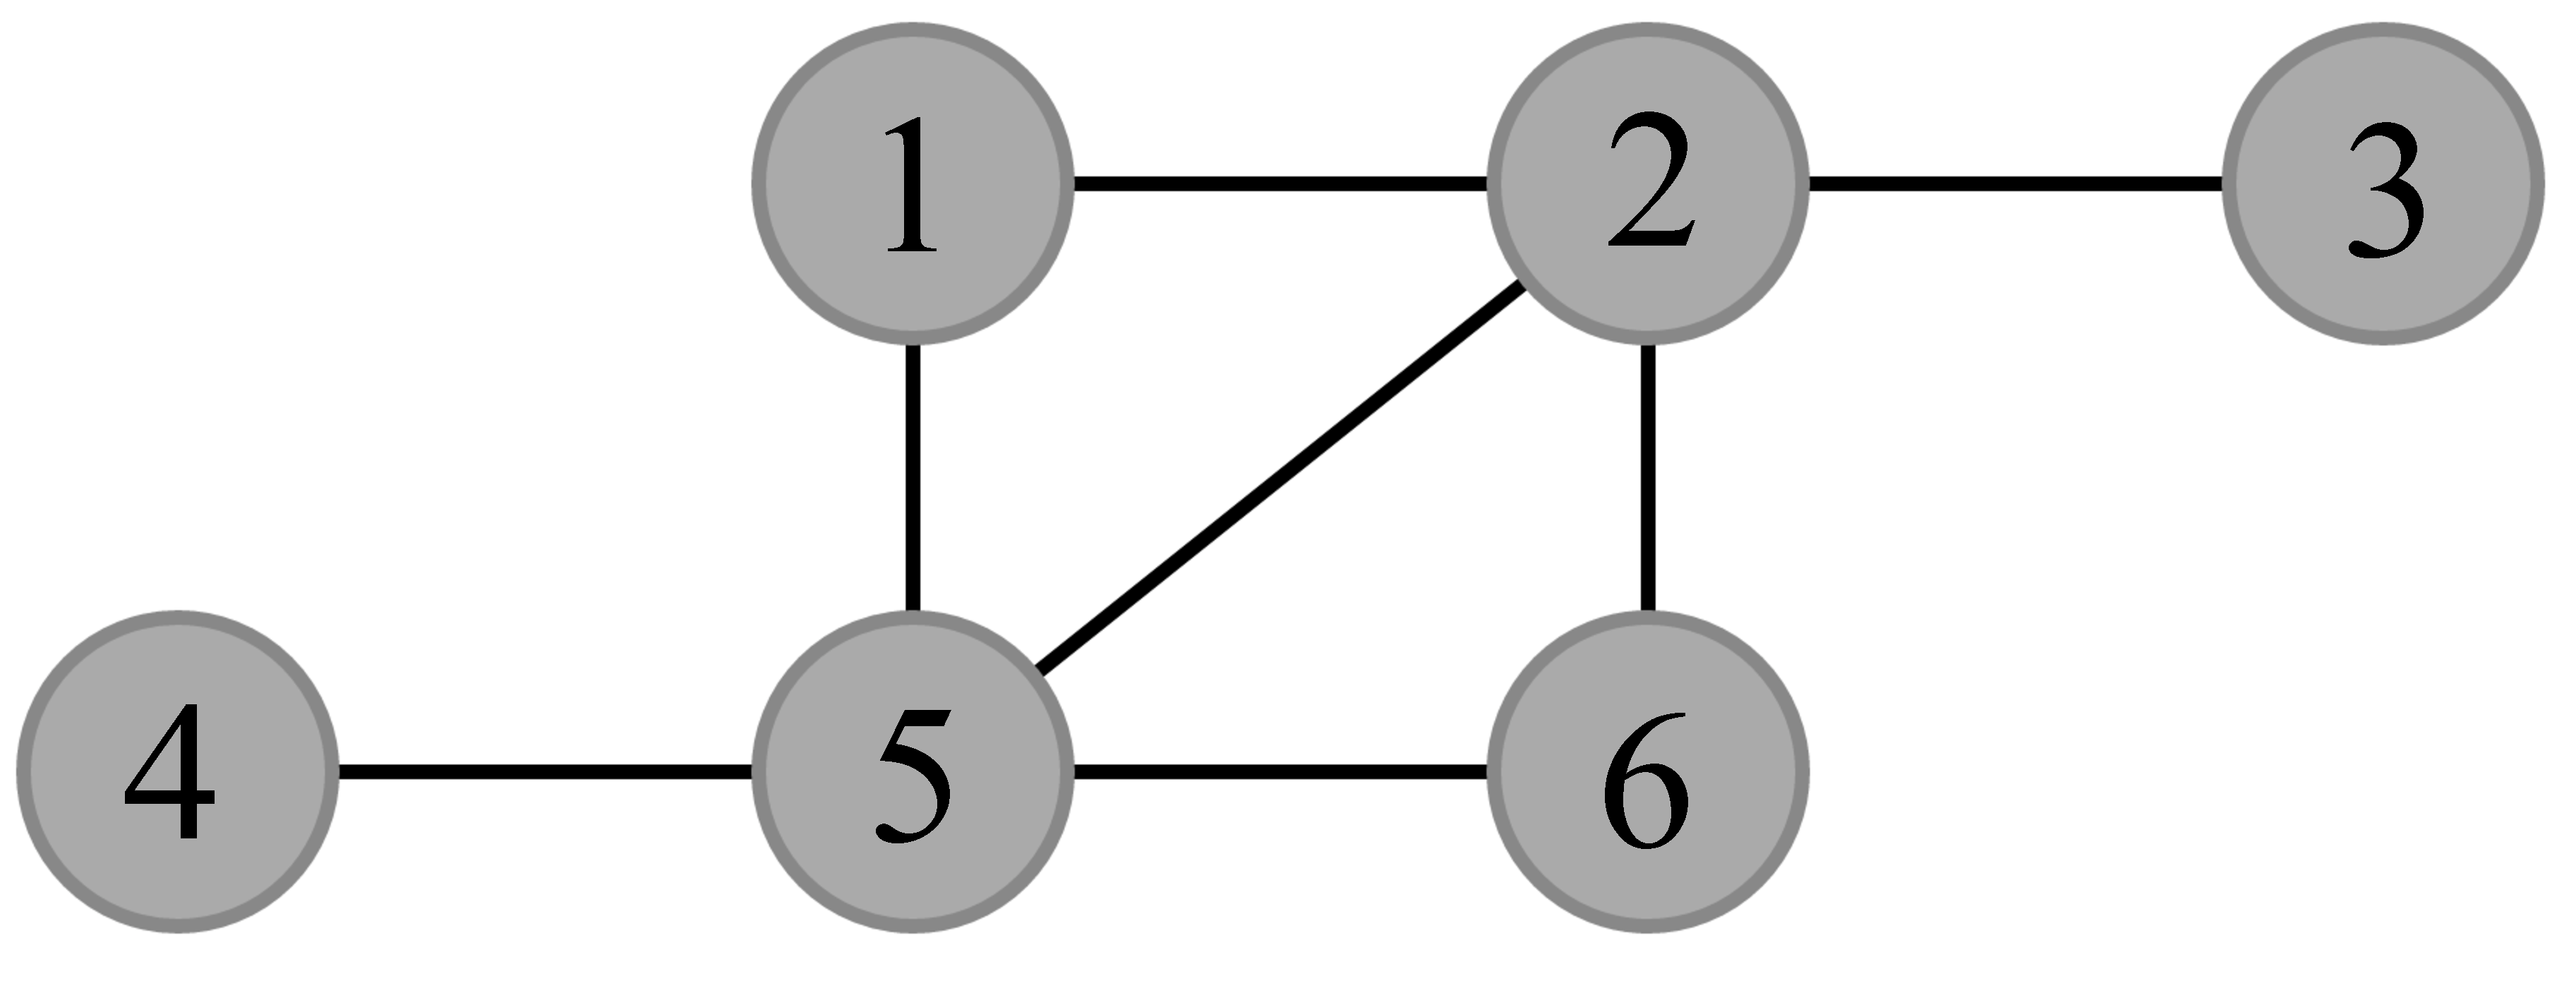
\includegraphics[width=7cm]{../figures/example.pdf}
	\caption{A simple, undirected graph $H$}\label{fig:graph}
\end{figure}

\subsection{Graph Theory}
\label{sec:graphtheory}

A graph, denoted $G=(V,E)$, is an ordered pair of two sets: a set of vertices $V$ and a set of edges $E$. Each edge consists of a pair of vertices from $V$. For example, $(u,w) \in E$ is an edge connecting vertices $u$ and $w$ where $u,w \in V$. Vertices are adjacent if they are connected by an edge. A simple graph is an undirected graph where each edge connects two different vertices and no two edges connect the same pair of vertices. All graphs used by the vertex coloring problem and conflict-free coloring problem will be undirected, simple graphs. An example graph that we will use later on is shown in figure \ref{fig:graph}.

The neighborhood of a vertex, denoted $N_G(v)$, is a set of all vertices adjacent to $v$. A \emph{closed} neighborhood consists of all vertices adjacent to $v$ and $v$ itself. Unless stated otherwise, we will assume when talking about neighborhoods that they are closed neighborhoods. The degree of a vertex, denoted $d_G(v)$, is the number of vertices adjacent to $v$. The maximum degree of a graph $G$, denoted $\Delta(G)$, is the maximum degree of its vertices. \cite{bondy1976graph}

\begin{figure}[h]
	\centering
	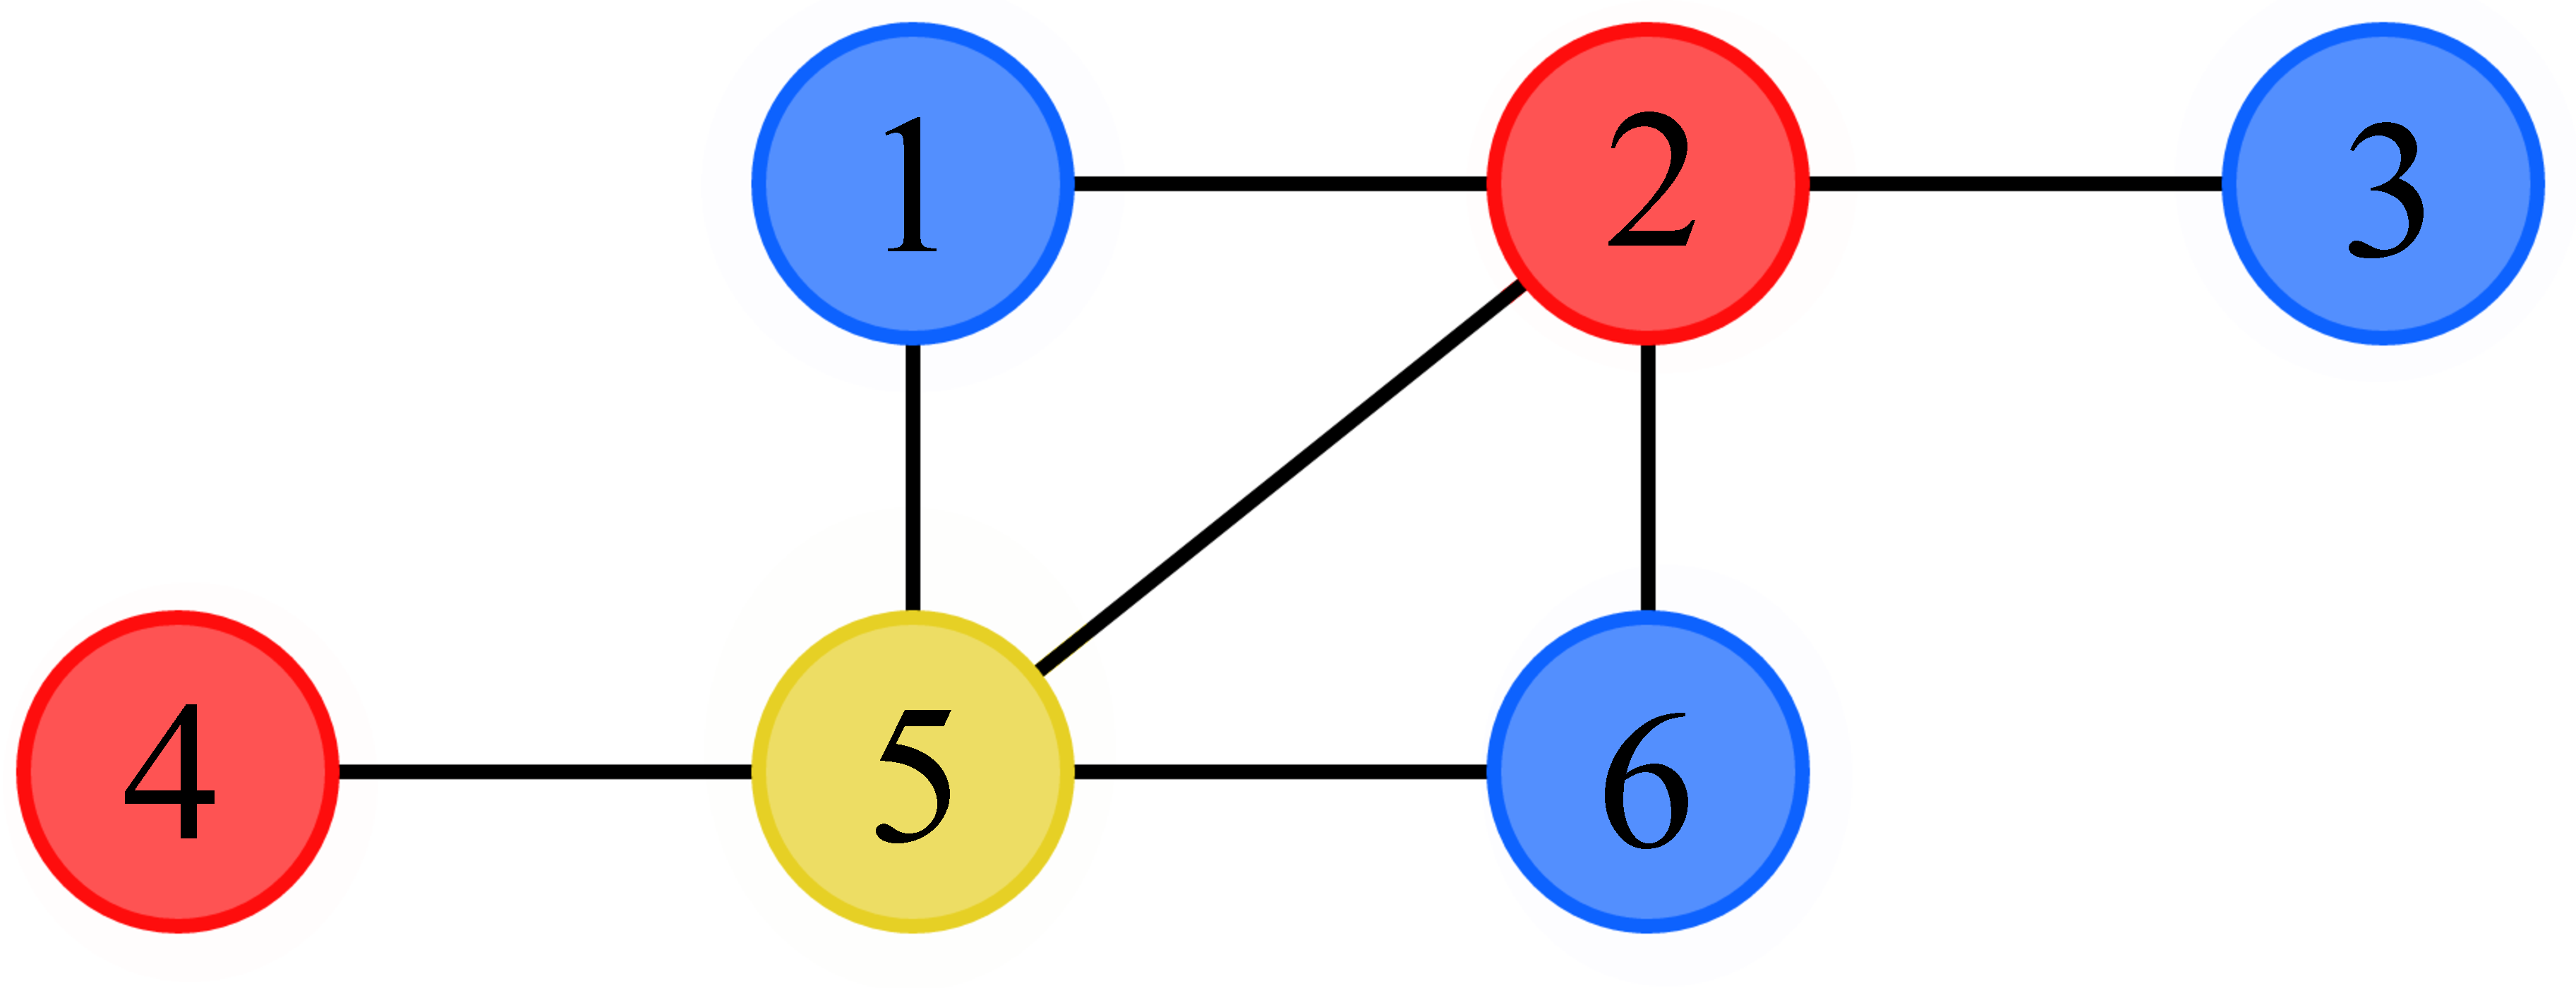
\includegraphics[width=7cm]{../figures/example-vcp.pdf}
	\caption{A minimum vertex coloring of $H$}\label{fig:vcp-example}
\end{figure}

\todo[inline]{The figures will be shaded with angled lines eventually}

\subsection{Graph Coloring}
\label{sec:coloring}
A vertex coloring is an assignment of colors to each vertex of a graph $G$ such that no adjacent vertices share the same color. Mathematically, it can be described as a function $f : V \rightarrow S = \{1, 2, \dots, k\}$ such that $\forall u,w \in V$, if $(u,w) \in E$, then $f(u) \neq f(w)$. A vertex coloring that satisfies this constraint is called a \emph{proper coloring}. The \emph{chromatic number} of $G$, denoted $\chi(G)$, is the minimum number of colors, i.e. $|S|$, needed to properly color $G$. The \emph{vertex coloring} problem, when given a simple graph $G$, is to find $\chi(G)$. \cite{bondy1976graph}

A graph $G$ is said to be \emph{k-colorable} if it can be colored using $k$ or fewer colors, i.e. $\chi(G) \leq k$. A graph having $\chi(G) = k$ is said to be a \emph{k-chromatic} graph. The \emph{k-colorability} problem asks if a graph can be colored using $k$ colors. This problem is a slightly easier problem than the vertex coloring problem as it is decision problem rather than an optimization problem. An example of a 3-colorable graph and a vertex coloring is shown in figure \ref{fig:vcp-example}.

\begin{figure}[h]
	\centering
	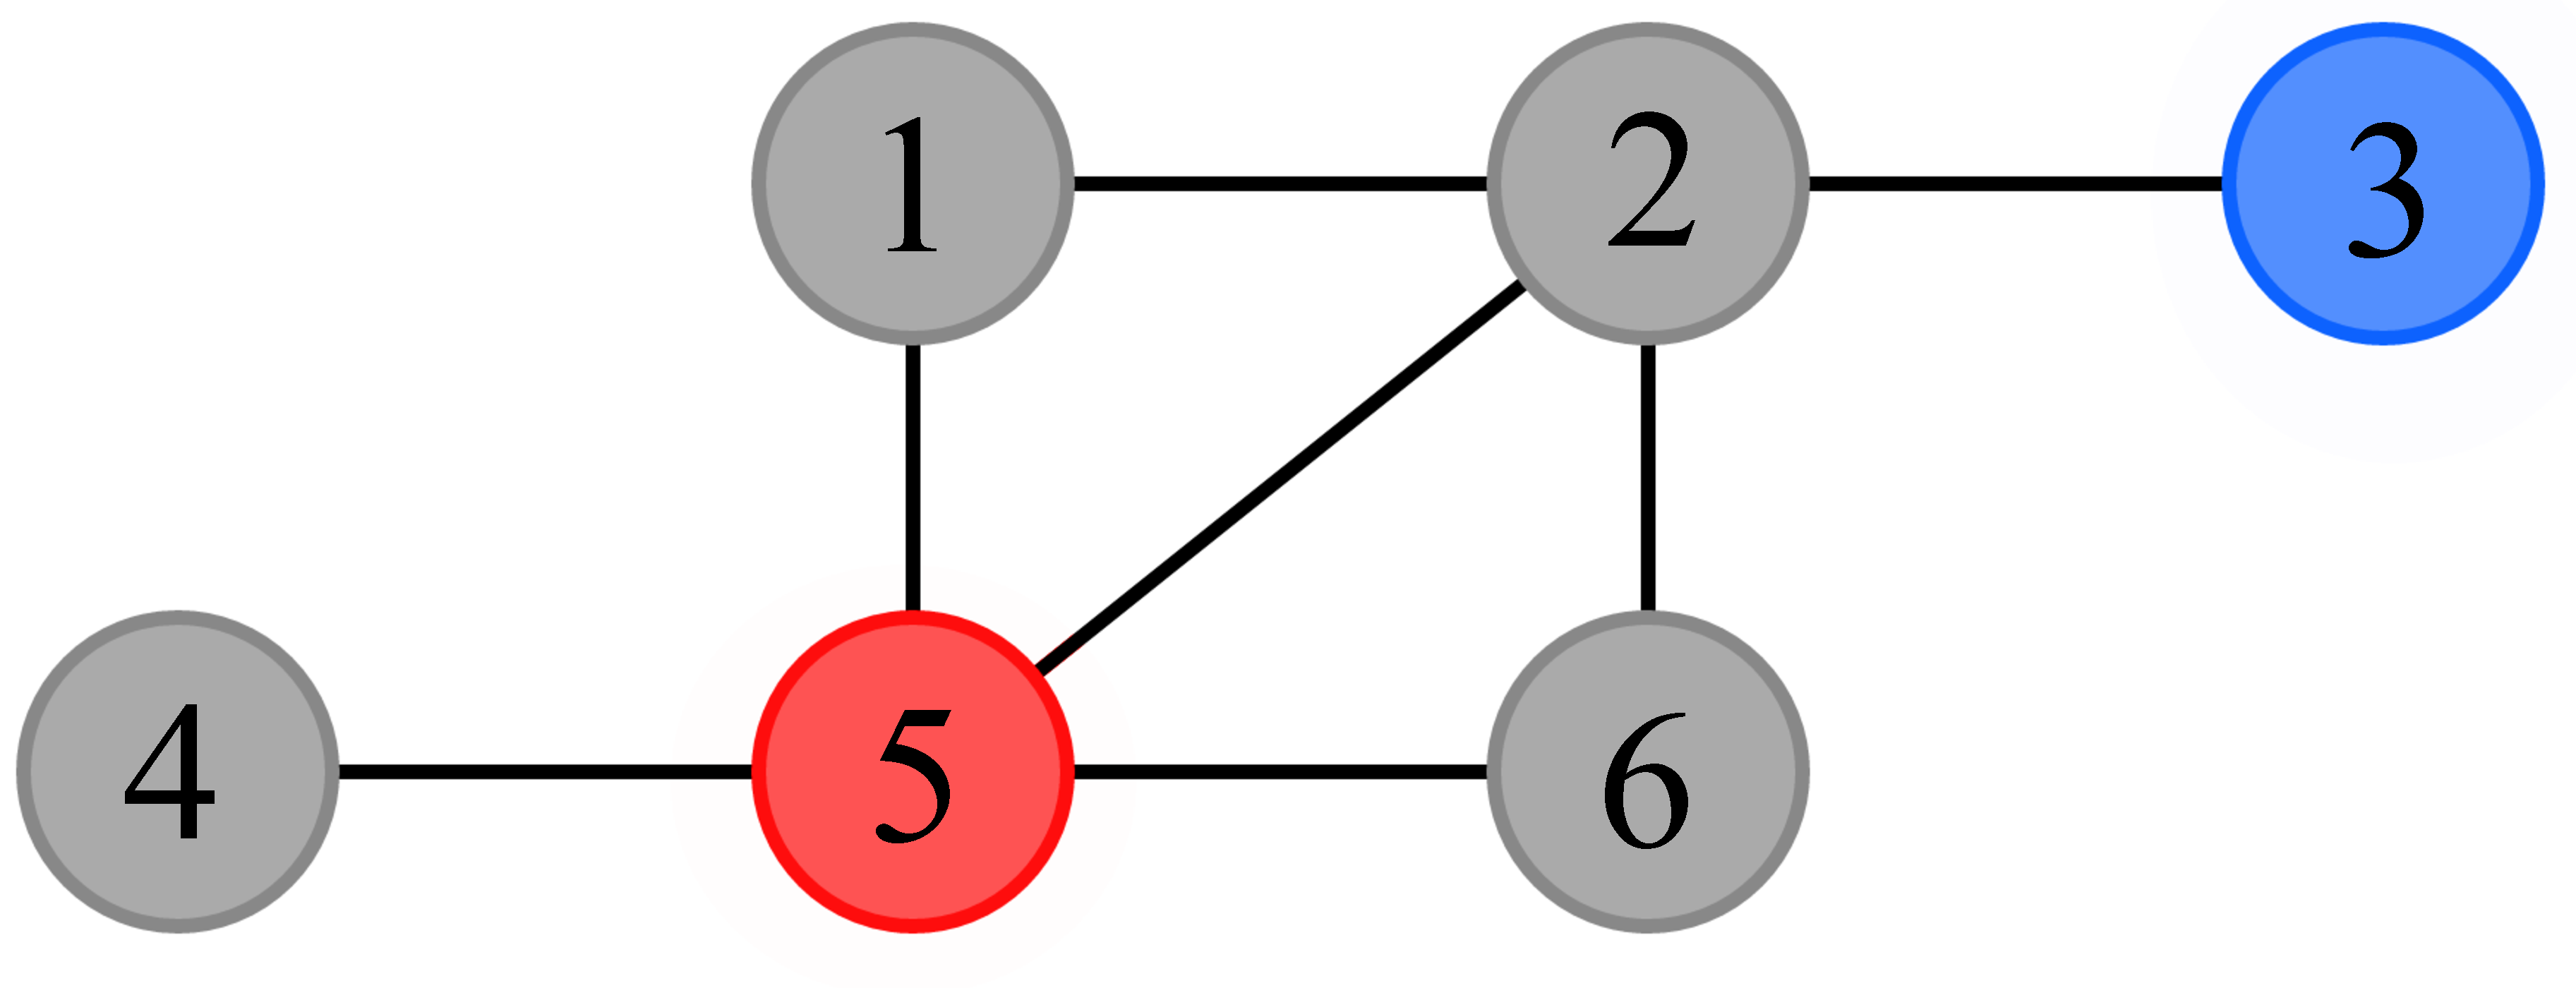
\includegraphics[width=7cm]{../figures/example-cfcp.pdf}
	\caption{A minimum conflict-free coloring of $H$}\label{fig:cfcp-example}
\end{figure}

A \emph{conflict-free coloring} of a graph assigns one of $k$ colors to some of the vertices such that, for every vertex $v$, there is a unique color assigned to a vertex among $v$ and $v$'s neighbors. A \emph{conflict-free k-coloring} of a simple graph $G$ assigns one of $k$ different colors to a subset $S \subseteq V$ of vertices such that $\forall v \in V$, there is a vertex $u \in N(v)$ where the color of $u$ is unique in the closed neighborhood of $v$. The vertex $u$ can be thought of the \emph{conflict-free neighbor} of $v$. The \emph{conflict-free chromatic number} of G, denoted $\chi_{CF}(G)$, is the smallest $k$ for which a conflict-free coloring exists. \cite{abel2017three}

An example of a conflict-free coloring is shown in figure \ref{fig:cfcp-example}. It is worth noting that all proper vertex colorings are also conflict-free colorings. This is because in a proper vertex coloring, every vertex is its own conflict-free neighbor \cite{abel2017three}. We observe from figures \ref{fig:vcp-example} and \ref{fig:cfcp-example}, $\chi(H) = 3$ and $\chi_{CF}(H) = 2$.

The domination number of $G$, denoted $\gamma(G)$, is the size of a minimum dominating set of G. A dominating set is a subset $D$ of $V$ such that every vertex not in $D$ is adjacent to at least one vertex in $D$. The \emph{conflict-free domination number} for some $k$, denoted $\gamma_{CF}^k(G)$, is the minimum number of vertices that have to be colored in a conflict-free k-coloring of $G$. An example of a dominating set is $\{3, 5\}$ of graph $H$ where $\gamma(H) = 2$.

\subsection{Computational Complexity Theory}
\label{sec:complexitytheory}
A \emph{decision} problem, as mentioned earlier, is a problem that can be answered with a `yes' or a `no' \cite{sipser2006introduction}. A decision problem is said to be in the class \emph{P} if in the worst case, it can be solved with an algorithm that runs in polynomial time. A problem can be solved in polynomial time if an algorithm with input size $n$ can run in at most $n^k$ steps where $k$ is a constant that does not depend on $n$.

Given a decision problem and information showing what the answer is, it can be possible to verify the answer quickly. If a decision problem can be verified in polynomial time but not necessarily solved in polynomial time, it is said to be in the class \emph{NP}. Take note that this does not exclude problems in class \emph{P}; \emph{P} is a subset of \emph{NP}.

There are certain problems that can be proven to be as hard as every problem in NP. There problems are said to be NP-hard. A problem is NP-hard if it every problem in NP can be polynomially reduced to it. This brings an important result: if an NP-hard problem can be solved with an algorithm that runs in polynomial time, then any problem in NP could be solved in polynomial time. A decision problem is said to be \emph{NP-complete} when it is both in NP and NP-hard.

The vertex coloring problem (VCP) and the conflict-free coloring problem (CFCP) are not in the class NP as they are not decision problems. A common approach to proving problems as NP-hard or NP-complete is a reduction from a known NP problem. If we find a known hard problem $Y$, then we can prove that another problem $X$ is hard by reducing $Y$ to $X$. The VCP and the CFCP have both been shown to be NP-hard \cite{abel2017three,moret1998theory}. The \emph{k-colorability} problem is proven to be NP-complete with a reduction from 3-SAT, a well-known NP-complete problem \cite{sharma2012new}.

\section{CF Coloring of General Graphs}
For the rest of this paper, we will consider the NP-complete problem of conflict-free k-colorability. Given a graph $G$ and an integer $k$, determine if graph $G$ can be colored using $k$ or fewer colors. Although all graphs can be conflict-free colored, a given graph $G$ may not be able to be colored with $k$ colors.

As shown with graph $H$ in section \ref{sec:background}, even though all proper vertex colorings are also conflict-free colorings, fewer colors can usually be used. This leads us to use heuristics that differ from the vertex coloring problem. Abel et al. \cite{abel2017three} present an efficient heuristic to color certain general graphs with $k$ colors in a conflict-free manner. They call this heuristic \emph{iterated elimination of distance-3-sets}.

\subsection{Guaranteeing CF k-Colorability}
It is wasteful to spend time coloring a graph that cannot be conflict-free colored with $k$ colors. This leads Abel et al. \cite{abel2017three} to provide sufficient criterion to guarantee the conflict-free k-colorability of a graph. To introduce this criterion, we need to define a few more terms.



\subsection{Iterated Elimination of Distance-3-Sets}

\begin{algorithm}
\caption{Iterated elimination of distance-3-sets} \label{alg:elimination}
\begin{algorithmic}[1]
\State $i \gets 1$, $\chi \gets \emptyset$
\State Remove all isolated paths from $G$
\While{$G$ is not empty}
	\State $D \gets \emptyset$
	\ForAll{components of $G$}
		\State Pick a vertex $v$ and add it to $D$
		\While{$\exists u$ at distance $\geq 3$ $\forall v \in D$}
			\State Pick $u$ at distance 3 from some vertex in $D$
			\State $D \gets D \cup \{ w \}$
		\EndWhile
		\ForAll{$u \in D$}
			\State Color $u$ with color $i$
		\EndFor
		\State $i \gets i + 1$
		\State Remove $N[D]$ from $G$
		\State Remove all isolated paths from G
	\EndFor
\EndWhile
\State Color all removed isolated paths using color $i$
\end{algorithmic}
\end{algorithm}


\section{CF Coloring of Planar Graphs}


\section{Complexity of Coloring CF Graphs}



\section{Conclusion}
\label{sec:conclusion}

\section{Acknowledgments}
\cite{abel2017three}


\bibliographystyle{abbrv}
\bibliography{../references}


\end{document}
